\documentclass{../../../fal_assignment}
\graphicspath{ {../../../} }

\usepackage{subcaption}

\hypersetup{
    colorlinks=true, 
    urlcolor=blue,
    linkcolor=
}

\usepackage{listings}
\lstset{
	basicstyle=\ttfamily,
	frame=single,
	showstringspaces=false,
	breaklines=false,
	prebreak={\space\hbox{\textcolor{gray}{$\hookleftarrow$}}}
}
\lstset{
	commentstyle=\ttfamily\textit,
	keywordstyle=\ttfamily\textbf,
	stringstyle=\ttfamily,
	rulecolor=\color{black}
}
\lstset{language=C++}

\title{Worksheet 3: Raycasting}
\author{Kate Bergel}
\module{COMP270}
\version{1.0}

\begin{document}

\maketitle

\section*{Introduction}

In this worksheet you will use 3D vectors and matrices to complete the implementation of a basic ray caster.

Begin by \textbf{forking} the following BitBucket repository:

\begin{center}
	\url{https://gamesgit.falmouth.ac.uk/projects/COMP270/repos/comp270-worksheet-3}
\end{center}

\textbf{Complete} the \textbf{FOUR} tasks described below, remembering to \textbf{commit} your work regularly.
To submit your work, open a \textbf{pull request} from your forked repository to the original repository.

\textbf{Note}: The tasks below can be completed by filling in the relevant functions marked in \texttt{Camera.cpp}, \texttt{Object.cpp} and \texttt{Matrix3D.cpp}, however you are welcome (and encouraged) to add helper methods and member data to these classes (and the \texttt{Plane} class, which derives from \texttt{Object}), expecially for Task 4. It should not be necessary to deviate from the main program structure; if you do decide to do so, your reasons should be stated in code comments and/or git commit messages.

Aside from the first task, which must be completed in order to actually see anything, the implementations do not depend on one another and may be attempted in any order.

\section*{Background}

\begin{figure}[ht]
	\begin{center}
		\begin{subfigure}[b]{0.45\linewidth}
			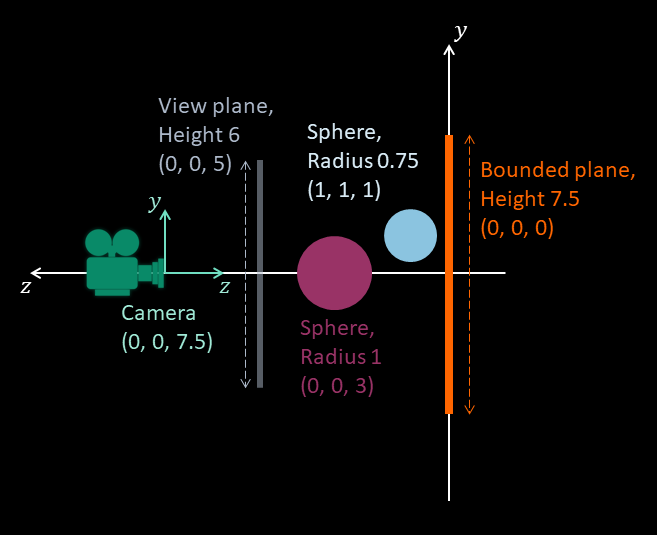
\includegraphics[width=\linewidth]{scene_side}
			\caption{Side view}
		\end{subfigure}
		\begin{subfigure}[b]{0.45\linewidth}
			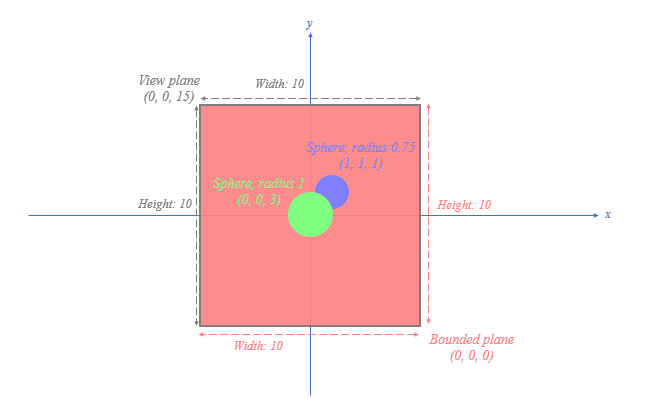
\includegraphics[width=\linewidth]{scene_top}
			\caption{Top view}
		\end{subfigure}
	\end{center}
	\caption{A diagram of the scene setup.}
	\label{fig:scene}
\end{figure}

The provided skeleton project implements a basic raycasting camera setup, as shown in Figure~\ref{fig:scene}.
The objects - two spheres and a plane - are already in the scene, though they cannot be seen to start with. The camera is initially at the point (0, 0, 20) in world space, facing along the negative \textit{z}-axis, and can be moved in a limited fashion, in directions along the world coordinate axes, with the following key presses:

\begin{itemize}
	\item \lstinline{a}: translates the camera in the negative \textit{x} direction ("left")
	\item \lstinline{d}: translates the camera in the positive \textit{x} direction ("right")
	\item \lstinline{s}: translates the camera in the negative \textit{y} direction ("up")
	\item \lstinline{w}: translates the camera in the positive \textit{y} direction ("down")
	\item \lstinline{q}:  translates the camera in the negative \textit{z} direction (towards the objects)
	\item \lstinline{e}:  translates the camera in the positive \textit{z} direction (away from the objects)
\end{itemize}

In addition, the camera can be "zoomed" in/out by pressing the up/down arrow keys, which moves the view plane away from/towards the camera.

\begin{marginquote}
``Happiness can be found, even in the darkest of times, if one only remembers to turn on the light."

\par --- Albus Dumbledore
\end{marginquote}

\section*{Task 1: let there be light}

The camera creates a picture by choosing a colour for each 'pixel' of the view plane based on which object in the scene is visible "through" the pixel's location in the view plane from the camera's position. The visibility test is carried out in \lstinline{Camera::updateScreenBuffer} by finding which objects are encountered by "rays" sent from the camera through the centre of each pixel. The number and directions of the rays will be determined by the view plane properties stored in the \lstinline{Camera::m_viewPlane} struct (\textbf{note}: the view plane distance is measured along the \textit{camera's viewing direction}).

\textbf{Implement} \lstinline{Camera::generateRays} to compute a unit-length \lstinline{Vector3D} direction for each ray and store it at the indices corresponding to the pixel it passes through in \lstinline{Camera::m_pixelRays} - you will need to make sure the data structure is sized appropriately!
\textbf{Note:} Pixel indices are assumed to correspond to the coordinate frame of the scene, where the \textit{y} axis points upwards, \textit{not} the SDL screen coordinates.

Once you've generated the rays, you should be able to see the spheres as in Figure~\ref{fig:spheres}.

\begin{figure}[ht]
	\begin{center}
		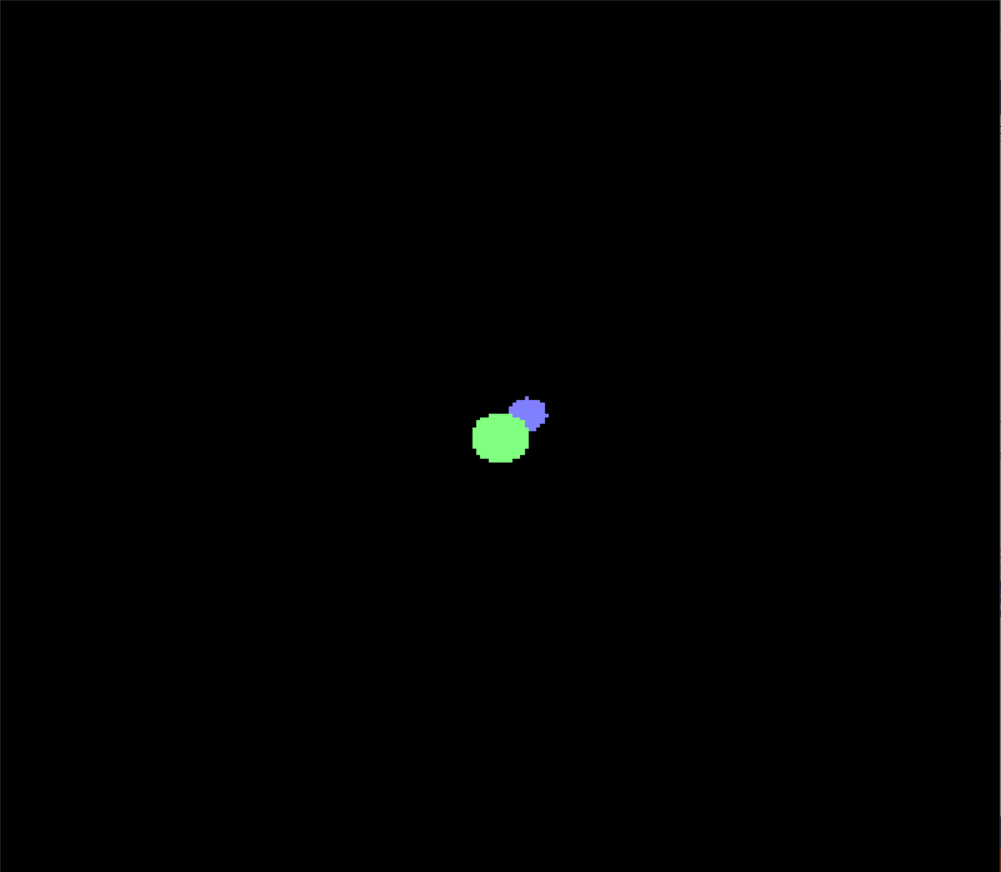
\includegraphics[width=0.25\linewidth]{spheres}
	\end{center}
	\caption{Scene view with ray generation.}
	\label{fig:spheres}
\end{figure}

\section*{Task 2: in plane sight}

There is another object in the scene that can't be seen yet, because the test to determine whether a ray intersects it is missing. \textbf{Implement} \lstinline{Plane::getIntersection} (in \texttt{Object.cpp}) to return \lstinline{true} if the ray intersects it within the bounds of its width and height, and set the input parameter \lstinline{distToFirstIntersection} to be the distance along the ray from its source that the intersection occurs.

Following this, your scene should look like Figure~\ref{fig:plane}.

\begin{figure}[ht]
	\begin{center}
		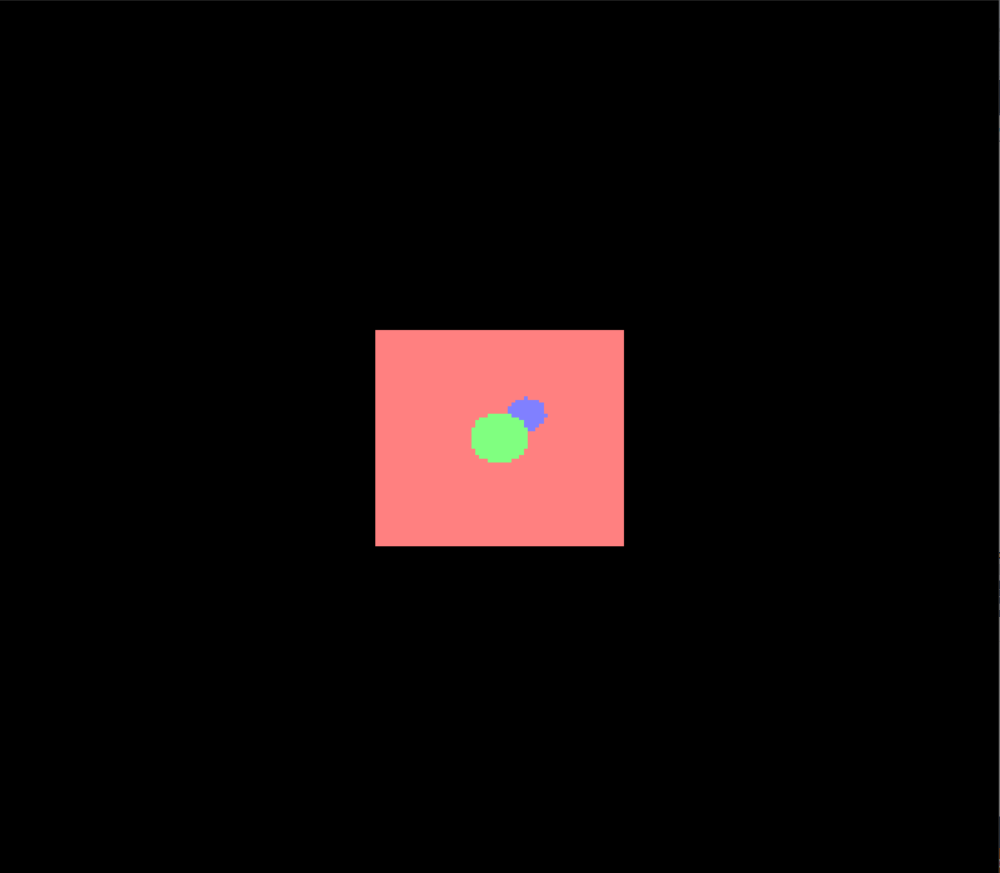
\includegraphics[width=0.25\linewidth]{plane}
	\end{center}
	\caption{Scene view with plane intersection.}
	\label{fig:plane}
\end{figure}

\section*{Task 3: spinning around}

Now you can see things, but only in a limited way, as the camera direction is fixed: although holding \texttt{shift} down when pressing the camera control keys modifies the values in \lstinline{Camera::m_rotation}, these values are not used when determining the scene layout relative to the camera. \textbf{Modify} \lstinline{Camera::updateWorldTransform} to compute the transform matrix that will transform the objects into camera space before the ray intersections are performed, and \lstinline{Matrix3D::inverseTransform} so that they can be transformed back again!

\textbf{Note:} there are various ways you in which you can perform the rotation, which may be relative to the camera (as a first person player view) or the world origin/other point of interest (as in a modelling tool such as Maya). Any solution is acceptable, provided it allows reasonably intuitive movement (you may edit the key mappings in \lstinline{Application::processEvent} if it helps) and preserves the proportions of the scene.

With rotations in place, you should be able to view the scene from more interesting angles, such as in  Figure~\ref{fig:rotate}.

\begin{figure}[ht]
	\begin{center}
		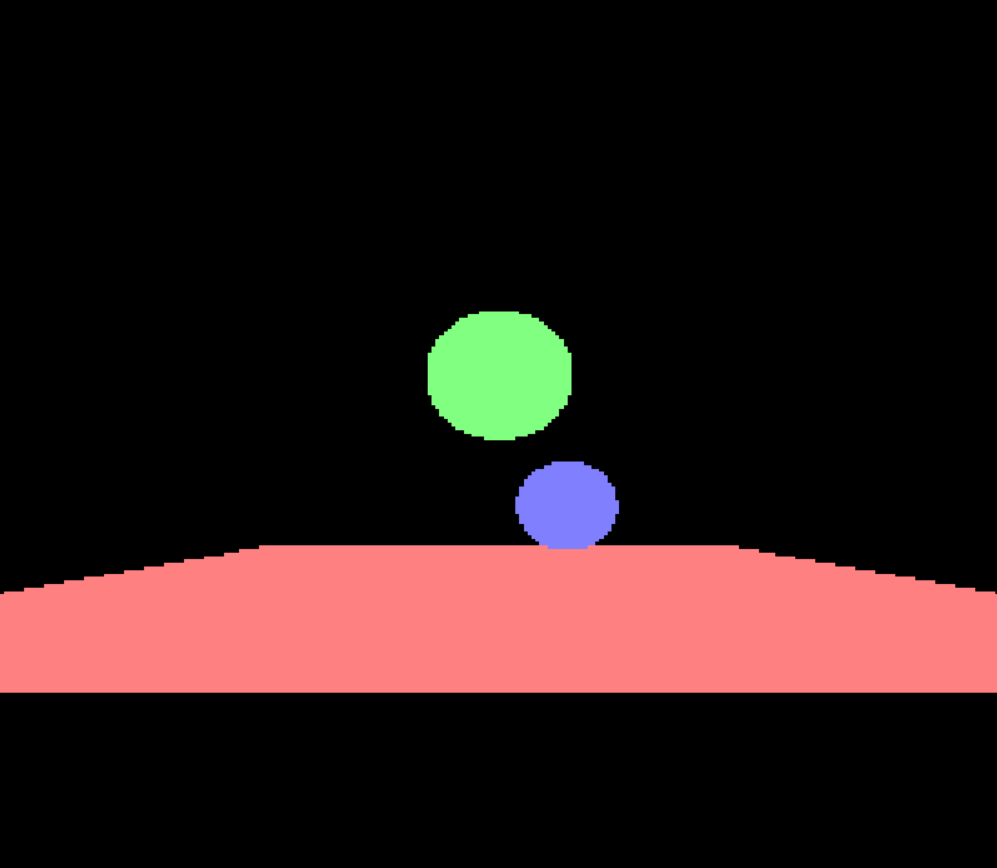
\includegraphics[width=0.25\linewidth]{rotate}
	\end{center}
	\caption{Scene view from a different angle.}
	\label{fig:rotate}
\end{figure}

\begin{marginquote}
``Unfortunately, no-one can be told what the Matrix is. You have to see it for yourself."

\par --- Morpheus
\end{marginquote}

\section*{Task 4: round things that look round}

So far, everything is looking rather flat because we're setting all the pixels to the same colour, regardless of "how much" they intersect the object. One way to add depth to a scene is to use \href{https://users.cs.northwestern.edu/~ago820/cs395/Papers/Phong_1975.pdf}{Phong shading}; shadows can also be created by sending rays that intersect an object back to a light source to see if any other objects block their path, and modifying the resulting pixel colour accordingly.

\textbf{Choose} (or \textbf{invent}) and \textbf{implement} a method for giving the scene a "more 3D" look - points will be awarded for creativity as well as adherence to existing techniques! You will almost certainly need to extend the functionality of more than one class; make sure to explain your chosen strategy and/or provide references to source material in the comments.

\rubrichead{All submissions and assessment criteria for this assignment are individual. To \textbf{pass} this assignment (achieve 40\% or more), you must submit a reasonable attempt at the worksheet by the formative deadline stated on LearningSpace.}
\begin{markingrubric}

	\firstcriterion{Basic competency threshold}{30\%}
		\grade\fail	A reasonable attempt at the worksheet was not submitted by the formative deadline.
		\par Evidence of breach of academic integrity.
		
    \criterion{PROCESS:\\Functional coherence}{40\%}
        \grade\fail None of the tasks have been attempted.
		\grade Task 1 has been attempted and partially completed.
		\grade Task 1 has been successfully completed.
		\grade Two tasks (including task 1) have been successfully completed.
		\grade Three tasks (including task 1) have been successfully completed.
		\grade All four tasks have been successfully completed.

    \criterion{PROCESS:\\Maintainability}{30\%}
        \grade \fail The code is only sporadically commented, if at all, or comments are unclear.
            \par Few identifier names are clear or inappropriate.
            \par Code formatting hinders readability.
        \grade The code is well commented.
            \par Some identifier names are descriptive and appropriate.
            \par An attempt has been made to adhere to a consistent formatting style.
             \par There is little obvious duplication of code or of literal values.           
        \grade The code is reasonably well commented.
            \par Most identifier names are descriptive and appropriate.
            \par Most code adheres to a sensible formatting style.
             \par There is almost no obvious duplication of code or of literal values.   
        \grade The code is reasonably well commented, with appropriate high-level documentation.
            \par Almost all identifier names are descriptive and appropriate.
            \par Almost all code adheres to a sensible formatting style.
             \par There is no obvious duplication of code or of literal values. Some literal values can be easily ``tinkered''. 
        \grade The code is very well commented, with comprehensive appropriate high-level documentation.
            \par All identifier names are descriptive and appropriate.
            \par All code adheres to a sensible formatting style.
             \par There is no obvious duplication of code or of literal values. Most literal values are, where appropriate, easily ``tinkered''.  
        \grade The code is commented extremely well, with comprehensive appropriate high-level documentation.
            \par All identifier names are descriptive and appropriate.
            \par All code adheres to a sensible formatting style.
            \par There is no duplication of code or of literal values. Nearly all literal values are, where appropriate, easily ``tinkered''.  
\end{markingrubric}

\end{document}
